\section{Introdução}
%\UseRawInputEncoding

\begin{frame}

\frametitle{Introdução}

\begin{itemize}
  \item O que são ponteiros em C?.
  \item Por que usar ponteiros?.
\end{itemize}


\end{frame}


%=======================================================

\begin{frame}
\frametitle{Declaração e Uso de Ponteiros}

\vspace{0.5cm}

\textbf{Características:}

\begin{itemize}
\item Declaração de um ponteiro.
\item Operador de endereço (\&): armazena o endereço de um valor.
\item Operador indireto (dereferenciação) (*): Aplicando o
operador * fornece o valor armazenado naquele endereço.
\end{itemize}

\vspace{0.5cm}


\end{frame}


%=============================================================
\begin{frame}
\frametitle{Ponteiros}

	\begin{figure}[h]
		\centering
		\includegraphics[width=0.85\textwidth]{Imagens/Imag03.png}
		%\caption*{Linguagem Python.}
	\end{figure}


\end{frame}

%=======================================================

\begin{frame}
\frametitle{Declaração e Uso de Ponteiros}

	\begin{figure}[h]
		\centering
		\includegraphics[width=0.85\textwidth]{Imagens/Imag01.png}
		%\caption*{Linguagem Python.}
	\end{figure}


\end{frame}


\section{Exemplos}



%=======================================================
\begin{frame}[fragile]{Operador de endereço}
\begin{block}{Exemplo 1}
\begin{lstlisting}
  int main() {
    int a = 6;
    int b = 8;
    
    printf("Valor de a= %d", a);
    printf(" e endereco de a= %d \n", &a);
    
    printf("Valor de b= %d", b);
    printf(" e endereco de b= %d", &b);
    return 0;
  }
\end{lstlisting}
\end{block}
\end{frame}


%=======================================================
\begin{frame}[fragile]{Exemplos}
\begin{block}{Exemplo 2}
\begin{lstlisting}
  int main() {
    int num = 42;
    int *ptr;
    ptr = &num;
    printf("Valor de num: %d\n", num);
    printf("Endereco de num: %p\n", &num);
    printf("Valor apontado por ptr: %d\n", *ptr);
    printf("Endereco armazenado em ptr: %p\n", ptr);
    return 0;
  }
\end{lstlisting}
\end{block}
\end{frame}




%=======================================================
\begin{frame}[fragile]{Operador de dereferenciação}
\begin{block}{Exemplo 3}
\begin{lstlisting}
  int main() {
    int a = 6; //declara uma variavel
    int *p_b ;//declara ponteiro para um int
    
    p_b=&a;// atribui endereco do int para o ponteiro
    
    //expressa valores de duas formas
    printf("Valores: a= %d", a);
    printf(" , *p_b= %d\n", *p_b);
    
    //expressa endereco de duas formas
    printf("Enderecos: &a= %d", &a);
    printf(" ,p_b= %d\n", p_b);
    
	//Usa ponteiro para mudar o valor
	*p_b=*p_b +1;
	printf("Agora a= %d\n", a);
    return 0;
  }
\end{lstlisting}
\end{block}
\end{frame}


%=============================================================
\begin{frame}
\frametitle{Ponteiros e vetores}

	\begin{figure}[h]
		\centering
		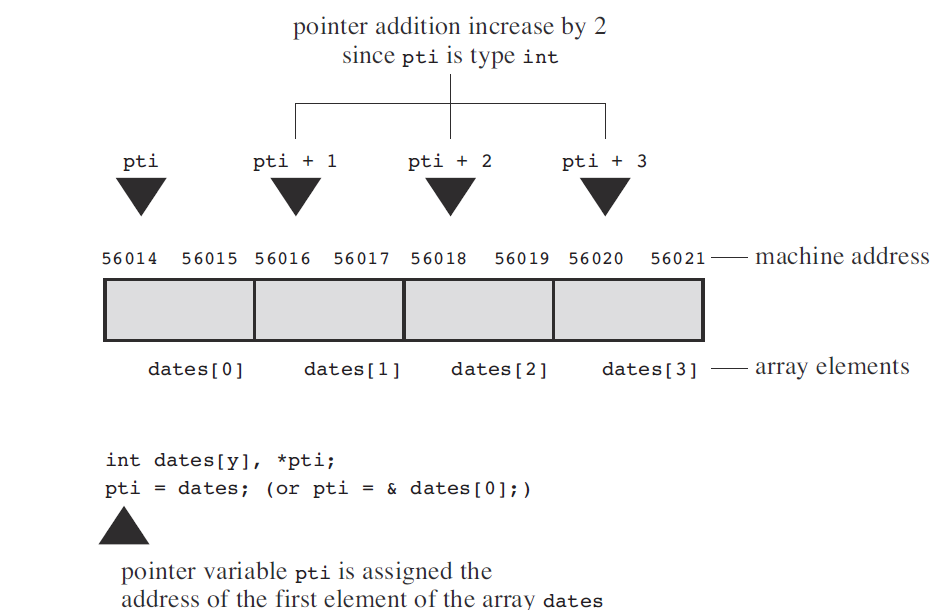
\includegraphics[width=0.85\textwidth]{Imagens/Imag02.png}
		%\caption*{Linguagem Python.}
	\end{figure}


\end{frame}


%=============================================================

\begin{frame}[fragile]
  \frametitle{Elementos de um vetor}
  \begin{block}{Exemplo 4}
  \begin{lstlisting}
  #include <stdio.h>
  int main() {
    int arr[] = {1, 2, 3, 4, 5};
    int *ptr = arr;
    printf("Endereco do array: %p\n",array);
    printf("Endereco do ponteiro: %p\n",&ptr);
    
    printf("Elemento %d\n", &arr[0]);
    printf("Elemento %d\n", &arr[1]);
    printf("Elemento %d\n", &arr[2]);
    printf("Elemento %d\n", &arr[3]);
    printf("Elemento %d\n", &arr[4]);
    
    
    printf("Elemento %d\n", *(ptr + 0));
    printf("Elemento %d\n", *(ptr + 1));
    printf("Elemento %d\n", *(ptr + 2));
    printf("Elemento %d\n", *(ptr + 3));
    printf("Elemento %d\n", *(ptr + 4));
        
    return 0;
  }
  \end{lstlisting}
  \end{block}
\end{frame}


%=============================================================

\begin{frame}[fragile]
  \frametitle{Soma dos elementos de um vetor}
  \begin{block}{Exemplo 5}
  \begin{lstlisting}
  #include <stdio.h>
  int main() {
    int arr[] = {1, 2, 3, 4, 5};
    int *ptr = arr;
    for (int i = 0; i < 5; i++) {
      printf("Elemento %d: %d\n", i, *(ptr + i));
    }
    return 0;
  }
  \end{lstlisting}
  \end{block}
\end{frame}


\section{Passagem por valor e por referência}

%============================================================


\begin{frame}[fragile]{}
  \frametitle{Usando funções por valor e por referência}
  \begin{block}{Exemplo 6: passando por valor}
  \begin{lstlisting}
  #include <stdio.h>
  int somar_valor(int,int);
  int main() {
    int a=5,b=4,c=0;

    c=somar_valor(a,b);
    printf("Resultado valor: %d\n",c);

    return 0;
  }
int somar_valor(int x,int y)
{
    int z=x+y;
    return z;

}  
  \end{lstlisting}
  \end{block}
\end{frame}

%============================================================

\begin{frame}[fragile]{}
  \frametitle{Usando funções por valor e por referência}
  \begin{block}{Exemplo 7: passando por referência}
  \begin{lstlisting}
  #include <stdio.h>
  void somar_ref(int*,int*);
  int main() {
  	int a=5,b=4;
    int *a_ptr=&a,*b_ptr=&b;
    somar_ref(a_ptr,b_ptr);
    printf("Resultado referencia: %d\n",*a_ptr);

    return 0;
  }
void somar_ref(int* x,int* y){
    *x=*x+*y;
}
  \end{lstlisting}
  \end{block}
\end{frame}

%============================================================


\begin{frame}{Referências}

\begin{itemize}
\item Prata, Stephen. C++ Primer Plus, 6th Edition. Índia: Pearson Education, 2012.
\item Prata, Stephen. C Primer Plus. Reino Unido: Pearson Education, 2013.
\end{itemize}





\end{frame}


